

\begin{figure*}[t]
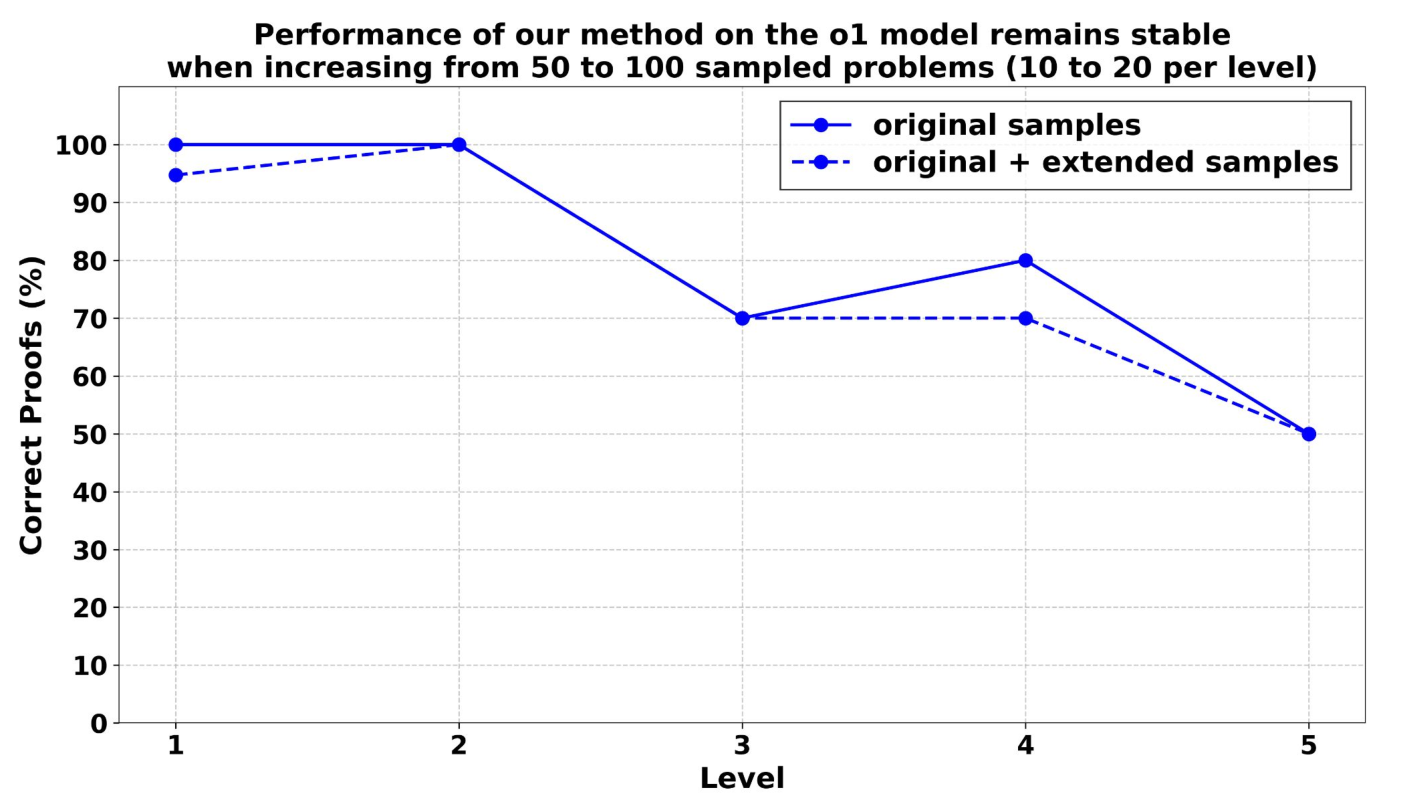
\includegraphics[width=0.99\textwidth]{latex/images/stability_of_results.pdf}
\centering
\caption{
Accuracy remains stable when increasing the sample size from 50 to 100 (10 additional problems per level), with an average variation of only 3\% per level. Per-level differences range from 0\% (levels 2, 3, and 5) to 5\% (level 1), and 10\% (level 4). We conclude our results are stable.
}
\label{fig:stability_of_results}
\end{figure*}


Figure~\ref{fig:stability_of_results} shows the performance of our method on both the original 50 samples and the extended set of 100 samples, broken down by level.
As shown, performance remains unchanged in levels 2, 3, and 5, while levels 1 show 5\% difference, and level 4 4 show a 10\% difference. Overall, the average difference across levels is 3\%. We conclude our results are stable.

We additionally repeat this stability check for the baseline (non-analogy) variant, on Gemini-Flash-2.5 and Claude Sonnet-4.6, given its substantially higher inference cost relative to our method (the baseline prompts with the full theorem dictionary rather than our analogy-derived, narrowed one). Baseline accuracy is similarly stable when increasing the evaluation set from 50 to 100 problems: for Gemini-Flash-2.5, overall accuracy increases only from 72\% to 74\%, with an average per-level variation of 6\%; for Claude Sonnet-4.6, overall accuracy increases only from 78\% to 80\%, with an average per-level variation of 4\%. These results confirm that our conclusions are robust to the evaluation sample size for both the proposed method and the baseline.